\documentclass[border=0.2cm]{standalone}
\usepackage{tikz}
\usetikzlibrary{calc}
\begin{document}


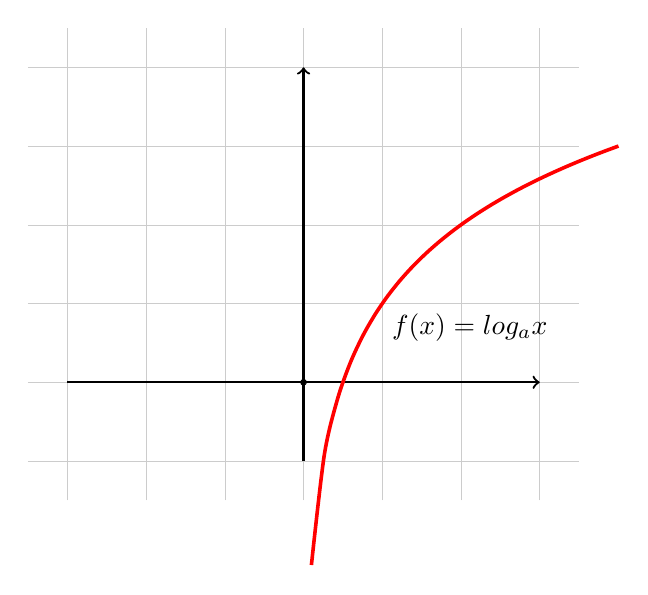
\begin{tikzpicture}
  \draw[help lines,black!20] (-3.5,-2.5) grid (3.5,3.5);
  \draw[thick,->] (-3,-1) -- (3,-1);
  \draw[thick,->] (0,-2) -- (0,3);
  \draw (0,-1) circle (1pt);
  \node[below right] at (1,0) {$f(x)=log_ax$};
  \draw[line width=1.3pt,red,domain=0.1:4,smooth,variable=\x] plot ({\x},{ln(\x)/ln(2)});
\end{tikzpicture}



\end{document}

